\documentclass[border=10pt]{standalone}
\usepackage{tikz}
\usetikzlibrary{arrows.meta,positioning}

\begin{document}
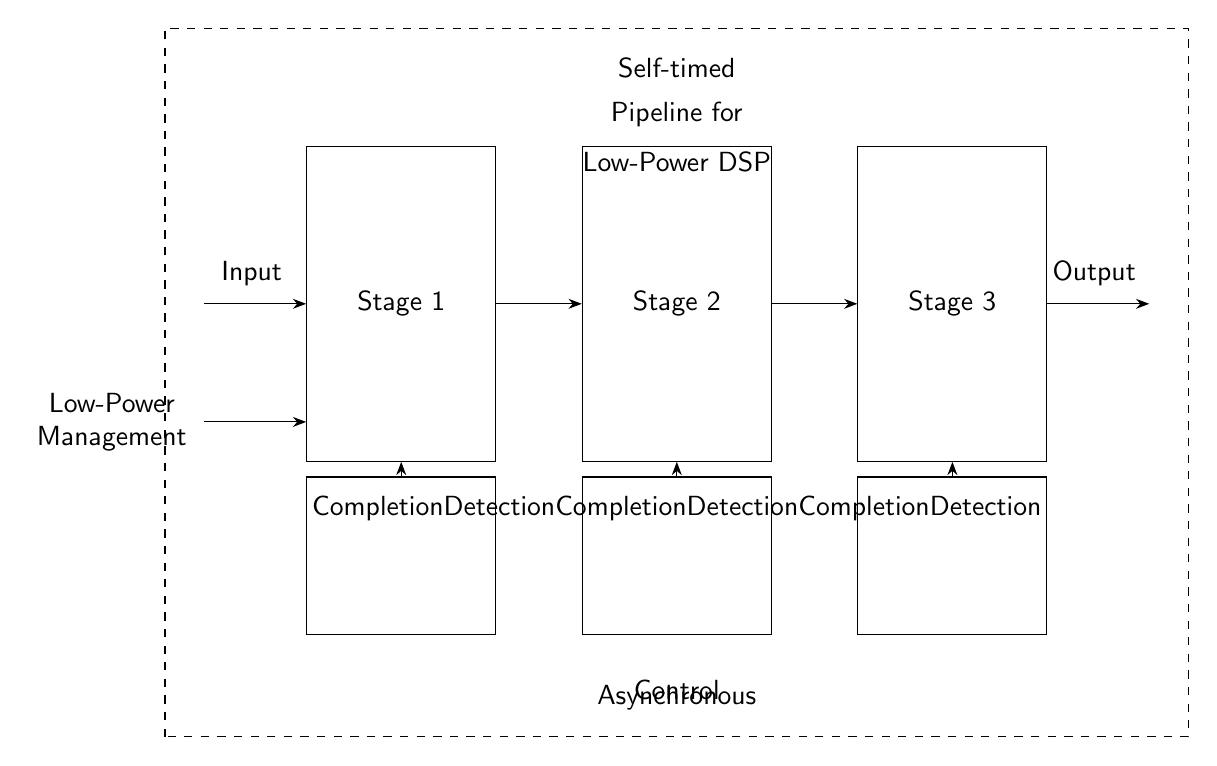
\begin{tikzpicture}[
    >=Stealth,
    block/.style={draw, minimum width=2.4cm, minimum height=4cm},
    smallblock/.style={draw, minimum width=2.4cm, minimum height=2cm},
    font=\sffamily
]

% Overall dashed frame
\draw[dashed] (-1.5,-4.5) rectangle (11.5,4.5);

% Top title (two/three lines)
\node[font=\sffamily] at (5,4) {Self-timed};
\node[font=\sffamily] at (5,3.4) {Pipeline for};
\node[font=\sffamily] at (5,2.8) {Low-Power DSP};

% Bottom title
\node[font=\sffamily] at (5,-4) {Asynchronous};
\node[font=\sffamily] at (5,-4.5+0.6) {Control};

% Stage blocks
\node[block] (s1) at (1.5,1.0) {};
\node[block] (s2) at (5,1.0) {};
\node[block] (s3) at (8.5,1.0) {};

\node at (s1) {Stage 1};
\node at (s2) {Stage 2};
\node at (s3) {Stage 3};

% Completion detection blocks
\node[smallblock] (c1) at (1.5,-2.2) {};
\node[smallblock] (c2) at (5,-2.2) {};
\node[smallblock] (c3) at (8.5,-2.2) {};

% Vertical arrows from completion detection to stages
\draw[->] (c1.north) -- (s1.south);
\draw[->] (c2.north) -- (s2.south);
\draw[->] (c3.north) -- (s3.south);

% Long completion detection text (to mimic overlapping words)
\node[font=\sffamily] at (5,-1.6) 
    {CompletionDetectionCompletionDetectionCompletionDetection};

% Horizontal arrows between stages
\draw[->] (s1.east) -- (s2.west);
\draw[->] (s2.east) -- (s3.west);

% Input arrow and label
\draw[->] (-1,1.0) -- (s1.west);
\node[anchor=south] at (-0.4,1.1) {Input};

% Output arrow and label
\draw[->] (s3.east) -- (11,1.0);
\node[anchor=south] at (10.3,1.1) {Output};

% Low-power management arrow and label (from left side)
\draw[->] (-1,-0.5) -- (s1.west |- -1,-0.5);
\node[anchor=east,align=center] at (-1.1,-0.5) {Low-Power\\Management};

\end{tikzpicture}
\end{document}